\documentclass[wide,a4paper,titlepage,12pt] {article}
\usepackage{polski}
\usepackage{float}
\usepackage[utf8]{inputenc}
\usepackage{listings}
\usepackage{slashbox}
\usepackage[table]{xcolor}
\usepackage{graphicx,pdflscape}
\usepackage{placeins}


\title{Technologie sieciowe 2}
\author{Tymon Tobolski (181037)\\ Jacek Wieczorek (181043)}

% Title page layout (fold)
\makeatletter
\renewcommand{\maketitle}{
\begin{titlepage}
  \begin{center}
    \vspace*{3cm}
    \LARGE \@title \par
    \vspace{2cm}
    \textit{\small Autor:}\par
    \normalsize \@author\par \normalsize
    \vspace{3cm}
    \textit{\small Prowadzący:}\par
    Dr inż. Arkadiusz Grzybowski\par
    \vspace{2cm}
    Wydział Elektroniki\\ III rok\\ Pn TN 11.15 - 13.00\par
    \vspace{4cm}
    \small \@date
  \end{center}
\end{titlepage}
}
\makeatother


\begin{document}
\maketitle
  \section{Cel laboratorium}
  \paragraph{}
  Celem laboratorium było opanowanie umiejętności konfiguracji sieci VLAN oraz łącza typu trunk w oparciu o protokól IEEE 802.1q na przełącznikach Cisco 2900.

  \section{Zadania}

  \subsection{Zestawienie sieci}
  \paragraph{}
  Zadanie polegało na zestawieniu sieci składającej się z jednego przełącznika oraz dwóch stacji roboczych.
  Z przydzielona puli adresów \textbf{10.4.0.64/27} stacje robocze otrzymały następujące adresy: PC1 - \textbf{10.4.0.66/27} oraz PC2 - \textbf{10.4.0.67/27}.
  \paragraph{}
  Stacje robocze zostały podłączone do przełącznika kablami prostymi.
  Połączenie między stacjami zostało zweryfikowane przy użyciu komendy \textbf{ping}.

  \begin{figure}[H]
    \begin{center}
      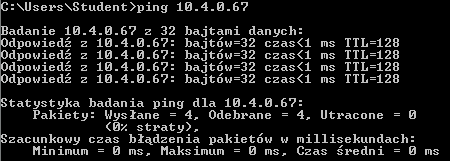
\includegraphics[width=\textwidth]{img/j1.PNG}
      \caption{Weryfikacja połączenia między stacją PC1 a PC2}
    \end{center}
  \end{figure}

  \begin{figure}[H]
    \begin{center}
      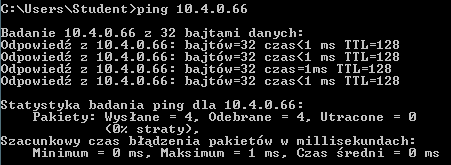
\includegraphics[width=\textwidth]{img/t1.PNG}
      \caption{Weryfikacja połączenia między stacją PC2 a PC1}
    \end{center}
  \end{figure}

  \begin{figure}[H]
    \begin{center}
      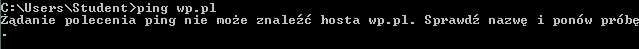
\includegraphics[width=\textwidth]{img/t2.PNG}
      \caption{Weryfikacja połączenia między stacją PC2 a Internetem}
    \end{center}
  \end{figure}

  \paragraph{}
  Na rysunkach 1 oraz 2 przedstawiono sposób weryfikacji połąćzenia między stacjami roboczymi PC1 i PC2. Wywołanie komendy \textbf{ping} w obu przypadkach zakonćżyło się pozytywnym rezultatem. W przypadku weryfikacji połączenia stacji roboczej PC2 z siecią Internet wynik był negatywny, co przedstawione jest na rysunku 3.

  \subsection{Podłączenie portu konsolowego}
  \paragraph{}
  Przełącznik został podłączony za pomocą kabla rollover do stacji roboczej PC2.

  Obecna konfiguracja przełącznika została usunięta za pomocą komend:
  \begin{verbatim}
    delete flash:vlan.dat
    erase startup-config
    reload
  \end{verbatim}

  Nazwa przełącznika (\textbf{S1}) została zmieniona za pomocą komendy:
  \begin{verbatim}
    hostname S1
  \end{verbatim}


  \begin{figure}[htbp]
    \begin{center}
      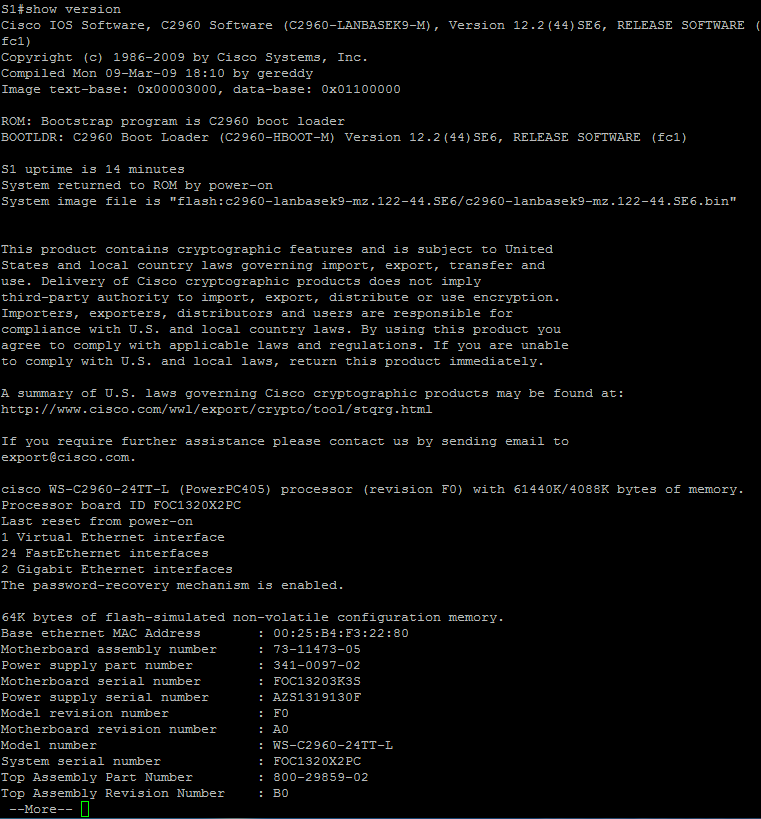
\includegraphics[width=\textwidth]{img/t3.PNG}
      \caption{Wynik polecenia \texttt{show version}}
    \end{center}
  \end{figure}

  \paragraph{}
  Polecenie \texttt{show version} pokazuje informacje dotyczące przełącznika takie jak: producent, model urządzenia, wersja oprogramowania, licencja producenta, czas od uruchomienia (uptime), dane dotyczące ilości i typu interfejsów, numery seryjne podzespołów.

  \begin{figure}[htbp]
    \begin{center}
      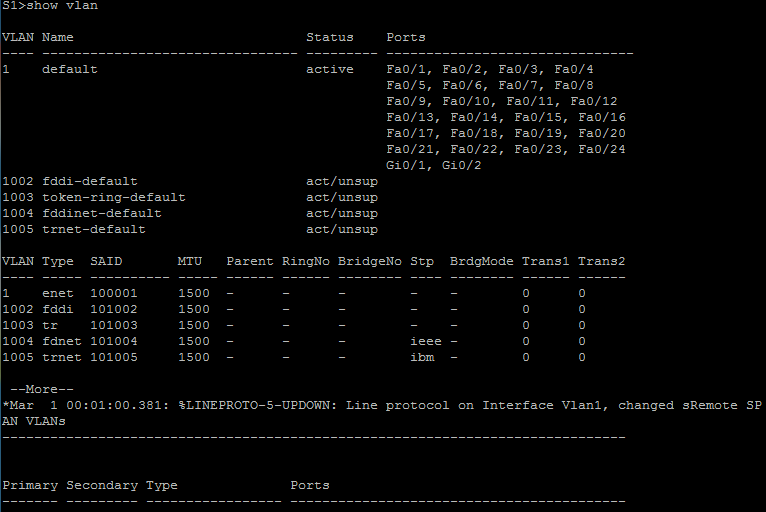
\includegraphics[width=\textwidth]{img/t4.PNG}
      \caption{Wynik polecenia \texttt{show vlan} na przełączniku S1}
      \label{fig:t4}
    \end{center}
  \end{figure}

  \paragraph{}
  Na Rysunku \ref{fig:t4} przedstawiona jest konfiguracja VLAN przełącznika po zresetowaniu konfiguracji startowej. Przełącznik posiada skonfigurowaną jedną sieć VLAN (domyślną), do której przypisane są wszystkie porty.


  \subsection{Tworzenie sieci VLAN}
  \paragraph{}
  W celu utworzenia dwóch sieci VLAN o nazwach \textbf{JacekWieczorek} i \textbf{TymonTobolski} na jednym przełączniku zostały wykonane następujące komendy:
  \begin{verbatim}
    S1(config)#vlan 10
    S1(config-vlan)#name JacekWieczorek

    S1(config)#vlan 11
    S1(config-vlan)#name TymonTobolski
  \end{verbatim}

  \paragraph{}
  Do powstałych sieci VLAN zostały dołączone porty przełącznika według Tabeli \ref{tab:t1}.
  Poniżej znajdują się komendy użyte do przypisania portów do odpowiednich sieci.

  \begin{verbatim}
    S1(config)#interface fa0/4
    S1(config-if)#switchport mode access
    S1(config-if)#switchport access vlan 10

    S1(config)#interface fa0/7
    S1(config-if)#switchport mode access
    S1(config-if)#switchport access vlan 10

    S1(config)#interface fa0/11
    S1(config-if)#switchport mode access
    S1(config-if)#switchport access vlan 10

    S1(config)#interface range fa0/14-22
    S1(config-if)#switchport mode access
    S1(config-if)#switchport access vlan 10
  \end{verbatim}


  \begin{table}[H]
    \begin{center}
      \begin{tabular}{|c|c|c|}
      \hline
      & VLAN 2 & VLAN 3 \\
      \hline
      S1 & 4,7,11 & 14-22 \\
      \hline
      S2 & 9-21 & 1,4,7 \\
      \hline
      \end{tabular}
    \end{center}
    \caption{Pula portów VLAN}
    \label{tab:t1}
  \end{table}

  \begin{figure}[H]
    \begin{center}
      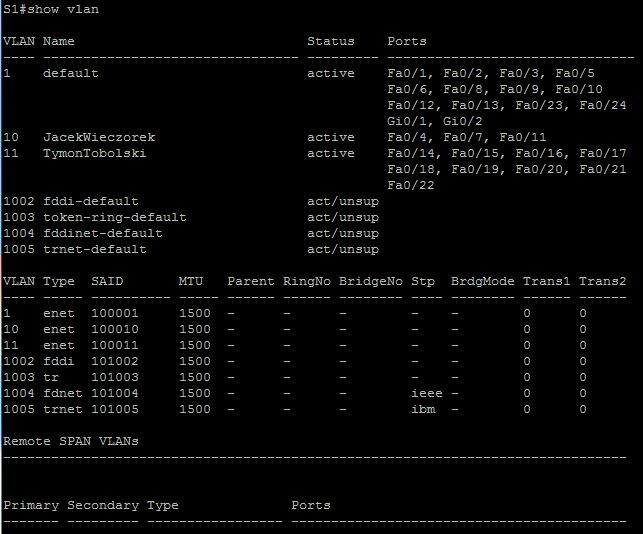
\includegraphics[width=\textwidth]{img/t6.PNG}
      \caption{Wynik polecenia \texttt{show vlan} na przełączniku S1}
      \label{fig:t6}
    \end{center}
  \end{figure}

  \paragraph{}
  Na Rysunku \ref{fig:t6} przedstawiona jest konfiguracja VLAN przełącznika S1 po utworzeniu dwóch sieci VLAN i przypisanie do nich portów zgodnie z Tabelą \ref{tab:t1}. Z domyślnej sieci VLAN wyłączone zostały porty, które zostały przypisane do sieci VLAN 10 i 11.

  \newpage
  \subsection{Weryfikacja połączenia}

  \begin{figure}[H]
    \begin{center}
      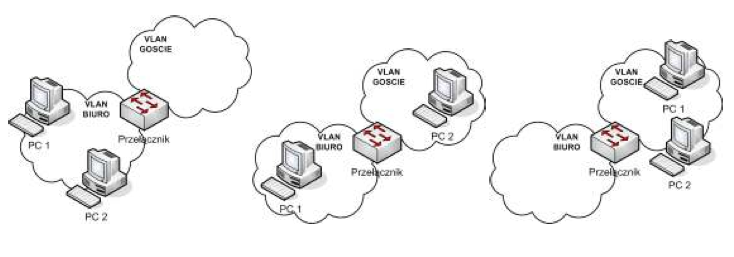
\includegraphics[width=\textwidth]{img/aa.PNG}
      \caption{Konfiguracje podłączenia stacji roboczych do przełącznika}
      \label{fig:aa}
    \end{center}
  \end{figure}

  \paragraph{}
  Na Rysunku \ref{fig:aa} przedstawiono trzy możliwe konfiguracje podłącznie stacji roboczych do przełącznika. W pierwszej i trzeciej sytuacji obie stacje robocze są podłączone do portów tej samej sieci VLAN. W takim wypadku weryfikacja połączenia międzu dwoma stacjami za pomocą komendy \textbf{ping} zakończyła się sukcesem. W drugim przypadku stacje robocze zostały podłączone do portów dwóch różnych sieci VLAN, co skutkowało niepowodzeniem weryfikacji połączenia miedzy stacjami.

  \subsection{Konfiguracja dodatkowego przełącznika}
  \paragraph{}
  Drugi przełącznik (\textbf{S2}) został skonfigurowany analogicznie jak pierwszy, według puli portów z Tabeli 1.

  \begin{figure}[H]
    \begin{center}
      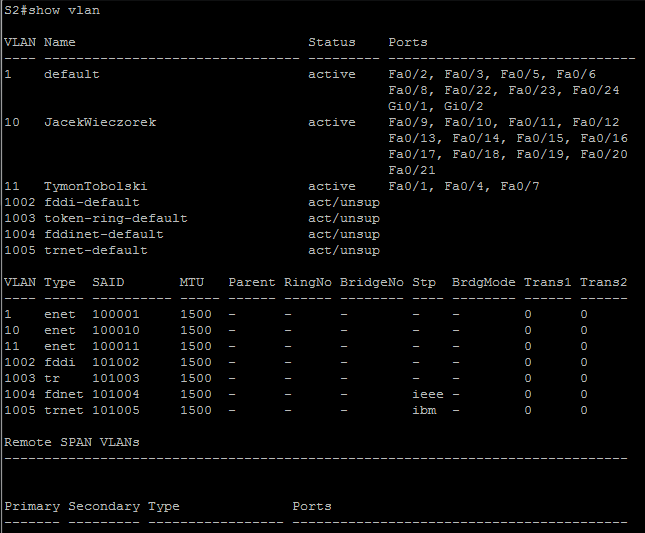
\includegraphics[width=\textwidth]{img/t8.PNG}
      \caption{Wynik polecenia \texttt{show vlan} na przełączniku S2}
      \label{fig:t8}
    \end{center}
  \end{figure}

  \paragraph{}
  Rysunek \ref{fig:t8} przedstawia wynik polecenia \texttt{show vlan} po zakończeniu konfiguracji przełącznika S2.

  \subsection{Konfiguracja łącza trunkowego pomiędzy dwoma przełącznikami}
  \paragraph{}
  Przełączniki zostały połączone za pomocą kabla z przeplotem (crossover) do portów FastEthernet 0/24.

  \begin{figure}[H]
    \begin{center}
      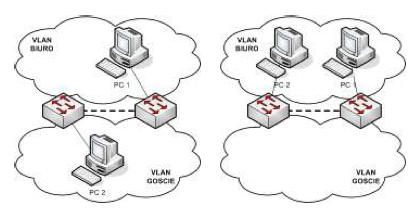
\includegraphics[width=\textwidth]{img/bb.PNG}
      \caption{Konfiguracje podłączenia stacji roboczych do przełączników}
      \label{fig:bb}
    \end{center}
  \end{figure}

  \paragraph{}
  Na Rysunku \ref{fig:bb} przedstawiono dwie możliwe konfiguracje podłączenia stacji roboczych do przełączników. W żadnej z wymienionych sytuacji weryfikacja połączenia między stacjami roboczymi zakończyłą się niepowodzeniem.

  \paragraph{}
  W celu skonfigurowania łącza typu \emph{trunk} na przełącznikach zostały wykonane następujące komendy.

  \begin{verbatim}
    S1(config)#interface fa0/24
    S1(config-if)#switchport mode trunk
  \end{verbatim}

  \begin{verbatim}
    S2(config)#interface fa0/24
    S2(config-if)#switchport mode trunk
  \end{verbatim}

  \paragraph{}
  Po skonfigurowaniu łącza typu \emph{trunk} weryfikacja połączenia między stacjami roboczymi w drugim przypadku (kiedy obie stacje były podłączone do tej samiej sieci VLAN) zakończyła się sukcesem. W przypadku podłączenia stacji roboczych do różnych sieci VLAN, weryfikacja połączenia ponownie zakończyła się niepowodzeniem.

  \begin{figure}[H]
    \begin{center}
      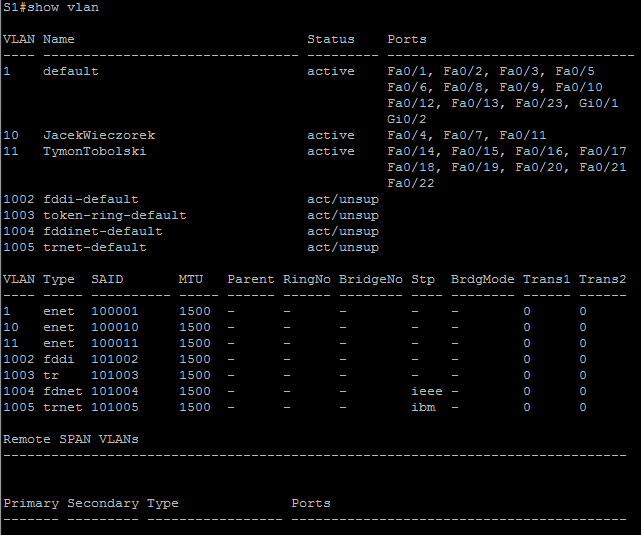
\includegraphics[width=\textwidth]{img/t9.PNG}
      \caption{Wynik polecenia \texttt{show vlan} na przełączniku S1 po konfiguracji połączenia trunk}
      \label{fig:t9}
    \end{center}
  \end{figure}

  \paragraph{}
  Rysunek \ref{fig:t9} przedstawia wynika polecenia \texttt{show vlan} na przełączniku S1 po konfiguracji połączenia trunk. Z domyślnej sieci VLAN wyłączony zostały port Fa0/24, który został skonfigurowany jako port łącza \emph{trunk}.

  \begin{figure}[H]
    \begin{center}
      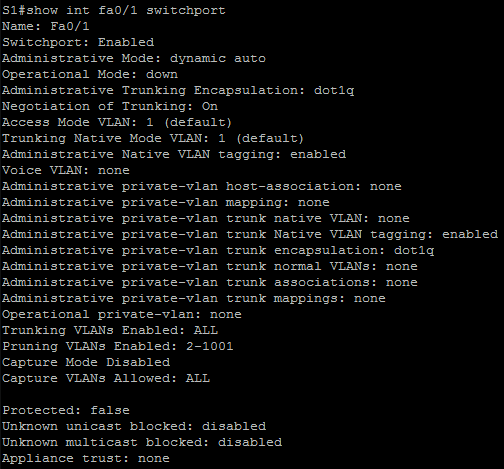
\includegraphics[width=\textwidth]{img/t10.PNG}
      \caption{Wynik polecenia \texttt{show int fa 0/1 switchport} na przełączniku S1 po konfiguracji połączenia trunk}
      \label{fig:t10}
    \end{center}
  \end{figure}

  \begin{figure}[H]
    \begin{center}
      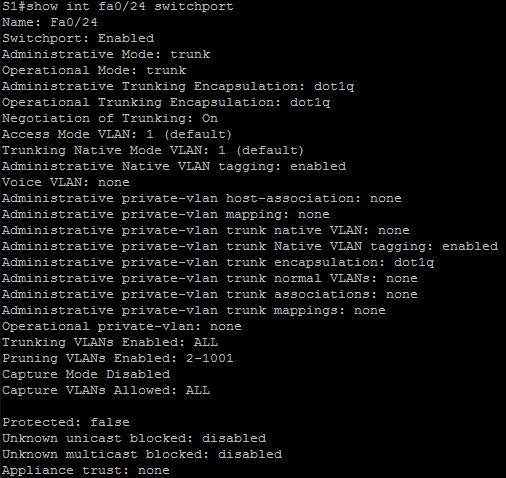
\includegraphics[width=\textwidth]{img/t11.PNG}
      \caption{Wynik polecenia \texttt{show int fa 0/24 switchport} na przełączniku S1 po konfiguracji połączenia trunk}
      \label{fig:t11}
    \end{center}
  \end{figure}

  \paragraph{}
  Analizaucjąc Rysunki \ref{fig:t10} oraz \ref{fig:t11} widać różnice w konfiguracji portów przełącznika. W przypadku portu \texttt{Fa0/1} tryb pracy został ustawiony jako \emph{dynamic auto}, natomiast w przypadku portu \texttt{Fa0/24} jako \emph{trunk}.


  \subsection{Konfiguracja z trzema przełącznikami}
  \begin{figure}[H]
    \begin{center}
      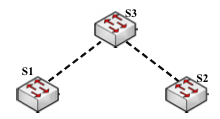
\includegraphics[width=\textwidth]{img/cc.PNG}
      \caption{Konfiguracja z trzema przełącznikami}
      \label{fig:cc}
    \end{center}
  \end{figure}

  \paragraph{}
  Na przełączniku S3 zostały skonfigurowane sieci VLAN oraz łącza \emph{trunk} na portach \texttt{Fa0/23} oraz \texttt{Fa0/24} za pomocą poniższych komend.

  \begin{verbatim}
    Switch(config)#interface fa0/23
    Switch(config-if)#switchport mode trunk

    Switch(config)#interface fa0/24
    Switch(config-if)#switchport mode trunk
  \end{verbatim}

  \paragraph{}
  Połączenie między przełącznikami S1 oraz S2 zostało rozłączone i zestawione według schematu na Rysunku \ref{fig:cc}.

  \paragraph{}
  Weryfikacja została przeprowadzaona identycznie jak w punkcie 2.6. Wyniki weryfikacji okazały sie zgodne z poprzednimi.



  \subsection{Analiza i konfiguracja protokołu STP}
  \begin{figure}[H]
    \begin{center}
      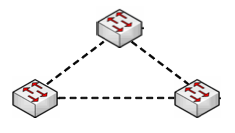
\includegraphics[width=\textwidth]{img/dd.PNG}
      \caption{Konfiguracja z trzema przełącznikami}
      \label{fig:dd}
    \end{center}
  \end{figure}

  \paragraph{}
  Przełączniki zostały podłączone zgodnie ze schematem na Rysunku \ref{fig:dd}.

  \begin{figure}[H]
    \begin{center}
      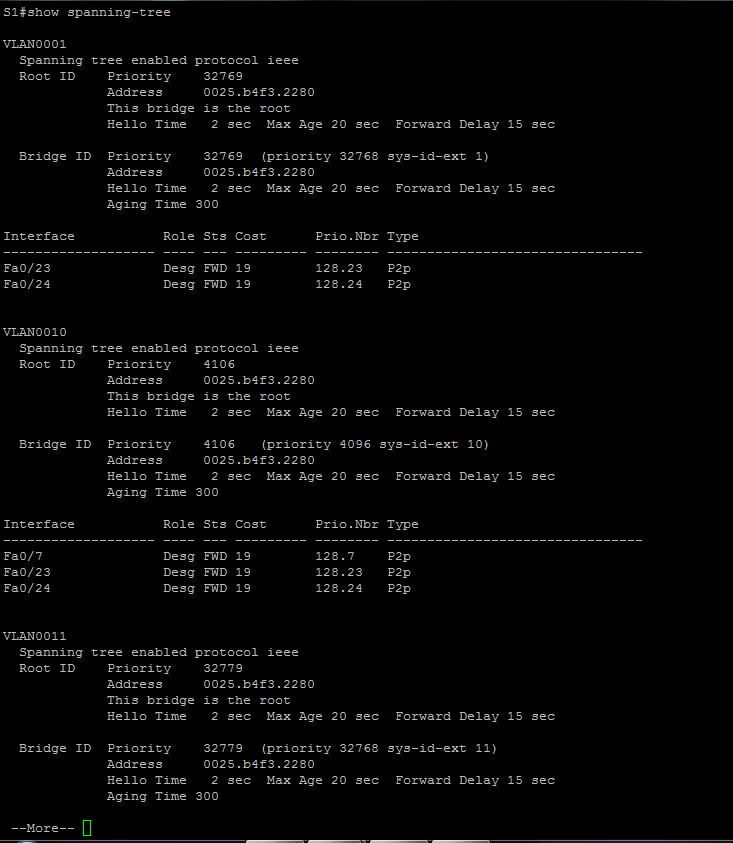
\includegraphics[width=\textwidth]{img/t13.PNG}
      \caption{Wynik polecenia \texttt{show spanning-tree} na przełączniku S1}
    \end{center}
  \end{figure}

  \paragraph{}
  
  Protokół Spanning-Tree jest protokołem wykorzystywantm w urządzenaich drugiej wartstwymodelu \textit{ISO$/$OSI}. 
  Został stworzony dla zwiększenia niezawodności ruchu sieciowego. Protokół ten tworzy graf bez pętli i ustala zapasowe łącza.
  Na szczycie grafu znajduje się korzeń (root). W momencie jak STP wykryje problem, rekonfiguruje sięć, uaktywniając łącza zapasowe.
  
  \paragraph{}
  Komenda \texttt{show spanning-tree} pokazuje skonfigurowane sieci VLAN. 
  Dla każdej sieci VLAN przedstawiona jest lista portów przypisanych do danej sieci, priorytet, adres węzła, mosty.


  \section{Wnioski}
  \paragraph{}
  W przypadku konieczności dynamicznych zmian w strukturze sieci najlepszym rozwiązaniem może okazać się odseparowania logicznej struktury sieci od struktury fizycznej za pomocą wirtualnych sieci LAN.
  Wirtualne sieci LAN znacznie ułatwiają przenoszenie stacji roboczych między podsieciami oraz dodawanie nowych stacji roboczych do instniejących już sieci. Usprawniają też nadzorowanie ruchu w sieci, a także poprawiają bezpieczeństwo.

\end{document}